\documentclass[12pt,letterpaper]{article}

%Packages
\usepackage{pdflscape}
\usepackage{fixltx2e}
\usepackage{textcomp}
\usepackage{fullpage}
\usepackage{natbib}
\usepackage{float}
\usepackage{latexsym}
\usepackage{url}
\usepackage{epsfig}
\usepackage{graphicx}
\usepackage{amssymb}
\usepackage{amsmath}
\usepackage{bm}
\usepackage{array}
\usepackage[version=3]{mhchem}
\usepackage{ifthen}
\usepackage{caption}
\usepackage{hyperref}
\usepackage{amsthm}
\usepackage{amstext}
\usepackage{enumerate}
\usepackage[osf]{mathpazo}
\usepackage{dcolumn}
\usepackage{lineno}
\pagenumbering{arabic}


%Pagination style and stuff
\linespread{2}
\raggedright
\setlength{\parindent}{0.5in}
\setcounter{secnumdepth}{0} 
\renewcommand{\section}[1]{%
\bigskip
\begin{center}
\begin{Large}
\normalfont\scshape #1
\medskip
\end{Large}
\end{center}}
\renewcommand{\subsection}[1]{%
\bigskip
\begin{center}
\begin{large}
\normalfont\itshape #1
\end{large}
\end{center}}
\renewcommand{\subsubsection}[1]{%
\vspace{2ex}
\noindent
\textit{#1.}---}
\renewcommand{\tableofcontents}{}
\bibpunct{(}{)}{;}{a}{}{,}

\section{Code}
All code for performing the analyses is available at: \url{https://github.com/TGuillerme/Total_Evidence_Method-Missing_data}.

\newpage
\section{Appendix 1: Tree Building}
  %\section{Supplementary material 1 : Tree building}

\subsection{Morphological character states}
To obtain a realistic value for the probability of having \textit{k} characters states for each simulated morphological character, we randomly selected 100 morphological matrices, each with more than 100 characters each, from TreeBASE (\url{http://treebase.org/}). We only selected matrices published between 1985 and 2013 and covering 19 taxonomic classes (Chordata, Arthropoda, Annelida, Angiosperm, Gymnosperm and Pteridophyta). This resulted in a total of 22563 characters that had between two and 10 character states. We then extracted the proportion of characters with each number of states (two to 10) to give us an empirical estimate of the average number of character states for each character, as shown in Figure \ref{Fig_AppendixCharacters}. Most characters have two or three states, therefore we only simulate characters with two or three states, and sample these in proportion to their occurrence in our empirical data (probability of 0.85 for two states characters and 0.15 for three state characters). The code used for this section is available at \url{https://github.com/TGuillerme/Total_Evidence_Method-Missing_data/blob/master/Analysis/MorphologicalCharacterStates.R}.

\begin{figure}
\centering
\includegraphics[keepaspectratio=true]{OnlineAppendices-LaTeXSuppFiles/SupplementaryFigures/TEM_Fig-AppendixCharacters.pdf}
\caption{The proportion of morphological characters with between two and 10 character states extracted from 100 randomly selected empirical matrices downloaded from TreeBASE.}
\label{Fig_AppendixCharacters}
\end{figure}

\newpage
\subsection{Tree Inference Software settings}

For clarity we have provided the exact settings used in our tree building below.

\subsubsection{Maximum Likelihood: RAxML version 8.0.20 \citep{Stamatakis21012014}}

\begin{itemize}
  \item Molecular data: GTR + $\Gamma_4$ (-m GTRGAMMA)
  \item Morphological data: Mk + $\Gamma_4$ (-K MK)
  \item Support: Rapid Boostrap algorithm (LSR), 1000 replicates
\end{itemize}

\subsubsection{Bayesian: MrBayes version 3.2.1 \citep{Ronquist2012mrbayes}}

\begin{itemize}
  \item Priors: Molecular data
  \begin{itemize}
    \item Rates distribution shape ($\alpha$) = 0.5
    \item Transition/Transversion ratio = 2 ($\beta$(80,40))
    \item Starting tree: "True" tree topology with each branch length = 1
  \end{itemize}
  \item Priors: Morphological data
  \begin{itemize}
    \item rates distribution shape ($\alpha$) = 0.5
  \end{itemize}
  \item Models
  \begin{itemize}
    \item Molecular data: HKY + $\Gamma_4$
    \item Morphological data: Mk + $\Gamma_4$
  \end{itemize}
  \item MCMC
  \begin{itemize}
    \item Two runs
    \item Four chains per run
    \item Generations $<$ 5$\times$$10^7$
    \item Sample frequency = 1.05$\times$$10^4$
    \item ASDS diagnosis frequency = 5$\times$$1^4$
    \item ASDS $<$ 0.01
    \item ESS $>>$ 200
    \item Burnin = 25\%
  \end{itemize}
\end{itemize}
  \label{Supp_TreeBuilding}

\newpage
\section{Appendix 2: Tree Comparisons}
  %\section{Supplementary material Section 2}

\subsection{Robinson-Foulds distance}
Robinson-Foulds distance (\textit{RF}; \citealp{RF1981}), or "path difference", measures the number of shared clades across two trees. The metric reflects the distance between the distributions of tips among clades in the two trees \citep{RF1981} and can be expressed as:
\begin{equation}
RF_{x,y} = N_{x} + N_{y} - 2C_{x,y}
\end{equation}
where $C_{x,y}$ is the number of clades in common in the two trees. $C$ is equal to one if the two trees have the same $n$ taxa; and $C = n-2$ when none of the $n$ taxa are shared between the trees. This metric is more sensitive to taxon displacement than Triplets distance (i.e. if one taxon moves out of a clade, then the clades are no longer considered similar; \citet{critchlowthe1996,johnson1998,wiensmissing2003}). The minimal value of $C$ is equal to 1 if the two trees have the same n taxa; the maximal value in $C = n-2$. For a fully unresolved tree (star tree) $N$=1 and for a fully resolved tree (binary tree) $N = n-2$. The minimal and maximal topological distance for taxa is:
\begin{equation}
RF_{min} = 1 + 1 - 2C_{x,y}
\end{equation}
and:
\begin{equation}
RF_{max} = 2(n-2)-2
\end{equation}
One can then rescale \textit{RF.scaled} by using the maximal and minimal value for any $n$ taxa:
\begin{equation}
RF.scaled_{x,y} = \frac{RF_{x,y}-RF_{max}}{RF_{max}}
\end{equation}
This metric is more sensitive to taxa displacement than the Triplets distance \citep{critchlowthe1996,johnson1998,wiensmissing2003} and therefore a low value will show a good clade conservation between two trees and a high value will show a bad recovery of common clades.

\subsection{Triplets distance details ($T_{x,y}$)}
Triplets distance ($T_{x,y}$; \citealp{dobson1975triplets}) measures the number of sub-trees made up of three taxa (triplets) that differ between two given trees. Each triplet can be written as $I_{ijk}$=(\textit{ijk}). Where $I_{ijk}$ is equal to zero if the the two triplets (\textit{ijk}) are the same in the two trees otherwise $I_{ijk}$ is equal to one. For any rooted binary tree there are only three possible combinations for each triplet: ((\textit{j},\textit{k}),\textit{i});, ((\textit{i},\textit{k}),\textit{j}); and ((\textit{i},\textit{j}),\textit{k}); \citep{johnson1998}. If the trees used are not fully binary, a fourth triplet combination is possible: (\textit{i},\textit{j},\textit{k}). We can calculate the triplet distance between two trees, $S_n$, as:
\begin{equation}
S_n = \sum_{ijk} I_{ijk}
\end{equation}
where:
\begin{equation}
\sum_{ijk} = \binom{n}{4} = \frac{n!}{4!(n-4)!}
\end{equation}
and where \textit{n} is the total number of taxa in both trees (modified from \citet{critchlowthe1996}). If $S_n$ = 0, the trees are identical; when $S_n$ = $\binom{n}{4}$, the trees are as different as possible (i.e. every taxon has a different placement in the two trees). Because the possible number of triplets per clade is a finite number, the probability of two random trees with the same $n$ taxa to have the same triplet is:
\begin{equation}
P({I_{ijk}}=0) = \frac{1}{4}
\end{equation}
Therefore one can calculate the probability of two random trees having the same triplets: 
\begin{equation}
P({S_{n}}=0) = \sum_{ijk} P_{I_{ijk}=0}
\end{equation}
\begin{equation}
P({S_{n}}=0) = \frac{n!}{4(3!(n-3)!}
\end{equation}
and in the same way:
\begin{equation}
P({S_{n}}=1) = \frac{3n!}{4(3!(n-3)!}
\end{equation}

\subsection{Normalised Tree Similarity}
For any tree with \textit{n} taxa compared using a tree distance metric $m$, Normalized Tree Similarity, $NTS_m$ \citep{Bogdanowicz2012}, represents the similarity score for the two trees given the expected distance between two random Yule trees with $n$ taxa. If $\bar{d}_{m,n}$\textit{(rand)} is the average distance between two random Yule trees with $n$ taxa and $d_{m,n}$\textit{(x,y)} the distance between the two trees \textit{x} and \textit{y} each containing $n$ taxa, then:
\begin{equation}
NTS_{m,n}(x,y)=\frac{\bar{d}_{m,n}(rand) - d_{m,n}(x,y)} {\bar{d}_{m,n}(rand)}
\end{equation}
\textit{NTS} ranges from one to -$\infty$.
For any $m,n$, when $NTS$ = 1, the trees are identical, when \textit{NTS} = 0 the trees are no more different than expected by chance, and when $NTS$ $<$ 0, the trees are more different than expected when comparing two random trees. 

We used the NTS method to scale all the Robinson Foulds and Triplets distances calculated in our analyses, using the TreeCmp java script \citep{Bogdanowicz2012}.

\subsection{Bhattacharyya Coefficient}
The Bhattacharyya Coefficient calculates the probability of overlap of two distributions \citep{Bhattacharyya}. When it is equal to zero, the probability of overlap of the distributions is also zero, and when it is equal to one, the two distributions are entirely overlapping. It forms an elegant and easy to compute continuous measurement of the probability of similarity between two distributions. The coefficient is calculated as the sum of the square root of the relative counts shared in \textit{n} bins among two distributions.
\begin{equation}
\text{Bhattacharyya Coefficient}=\sum_{i=1}^{n} \sqrt{{\sum{a_i}}\times{\sum{b_i}}}
\end{equation}
where
\begin{equation}
\sum{a_i}=\frac{\text{Number of counts in bin \textit{i} for the distribution \textit{a}}}{\text{Total number of counts for the distribution \textit{a}}}
\end{equation}
and
\begin{equation}
\sum{b_i}=\frac{\text{Number of counts in bin \textit{i} for the distribution \textit{b}}}{\text{Total number of counts for the distribution \textit{b}}}
\end{equation}
The precision of the Bhattacharyya Coefficient is directly related to the number of bins, $n$. If $n$ is low, the overlap will be overestimated and if $n$ is too high, the overlap will be underestimated. In this analysis, we determined the number of bins using Silverman's rule of thumb which states that $n$ should be 0.9 times the minimum of the standard deviation and the interquartile range of the distribution, divided by 1.34 times the sample size of the distribution to the negative one-fifth power (bw.nrd0() function in R; \citet{silverman1986density}).

  \label{Supp_TreeComparison}

\bibliographystyle{sysbio}
\bibliography{Supp_Ref}

\newpage
\section{Appendix 3: Additional Results}
  The following section contains the supplemental results of the effects of our missing data parameters and the different tree inference methods on the the ability to recover the "best" topology that are briefly discussed in the main body of the paper. For clarity, in the paper, we focused on the results of the effects of our missing data parameters on the Maximum Likelihood trees topology and the Bayesian consensus trees topology. The following additional results presented here give a greater insight into the effect of our missing data parameters on the Maximum Likelihood Bootstrapped trees topologies and the Bayesian posterior trees distribution topologies. Also we present here the pairwise comparisons between each parameters states for the Maximum Likelihood tree topology, the Maximum Likelihood Bootstrapped trees topologies and the Bayesian posterior trees distribution topologies.

\begin{figure} 
\centering
    \includegraphics[width=1\textwidth]{OnlineAppendices-LaTeXSuppFiles/SupplementaryFigures/Boot+Bayt-AllParam-RF+Tr-BW.pdf}
    \caption{Effect of increasing missing data on topological recovery using Maximum Likelihood Bootstrap trees (black) and Bayesian posterior tree distribution (grey). The x axis shows the percentage of missing data from 0\% (white) to 75\% (black) for the three parameters: $M_{L}$ (upper line), $M_{F}$ (middle line) and $M_{C}$ (lower line). Topological recovery was measured using two different tree comparison metrics: Normalised Robinson-Foulds distance (upper row) and Normalised Triplets distance (lower row). The graph shows the modal value (points), and the 50\% (thick solid lines) and 95\% (thin dashed lines) confidence intervals of the distributions of the tree comparison metric for each missing data parameter and tree inference method.} 
\label{Fig_Supp_BootBayt_allparam} 
\end{figure}

\begin{figure} 
\centering
     %Hide this figure for 'fast' build
%    \includegraphics[width=1\textwidth]{Figures/Supplementary/PairwiseComp-ML-RF+Tr-colour.pdf}
    \includegraphics[width=1\textwidth]{OnlineAppendices-LaTeXSuppFiles/SupplementaryFigures/PairwiseComp-ML-RF+Tr-colour.png} %bitmap version - 300 dpi RGB
    \caption{The effects of missing data on topological recovery using Maximum Likelihood trees. The x and the y axes both show show the percentage of missing data from 0\% (white) to 75\% (black) for the three parameters: $M_{L}$ (upper line), $M_{F}$ (middle line) and $M_{C}$ (lower line). Topological recovery is represented by the probability of (A) Normalised Robinson-Foulds distance and (B) Normalised Triplets distance distributions overlapping with the "best" tree distribution, calculated using the Bhattacharyya Coefficient. The Bhattacharyya Coefficient values are indicated using a color gradient ranging from low probability of overlap in blue, to a high probability of overlap in orange.}
\label{Fig_Supp_paircomp_ML}
\end{figure} 

\begin{figure} 
\centering
     %Hide this figure for 'fast' build
%    \includegraphics[width=1\textwidth]{Figures/Supplementary/PairwiseComp-Boot-RF+Tr-colour.pdf}
    \includegraphics[width=1\textwidth]{OnlineAppendices-LaTeXSuppFiles/SupplementaryFigures/PairwiseComp-Boot-RF+Tr-colour.png} %bitmap version - 300 dpi RGB
    \caption{The effects of missing data on topological recovery using Maximum Likelihood bootstrap trees. The x and the y axes both show show the percentage of missing data from 0\% (white) to 75\% (black) for the three parameters: $M_{L}$ (upper line), $M_{F}$ (middle line) and $M_{C}$ (lower line). Topological recovery is represented by the probability of (A) Normalised Robinson-Foulds distance and (B) Normalised Triplets distance distributions overlapping with the "best" tree distribution, calculated using the Bhattacharyya Coefficient. The Bhattacharyya Coefficient values are indicated using a color gradient ranging from low probability of overlap in blue, to a high probability of overlap in orange.}
\label{Fig_Supp_paircomp_Boot}
\end{figure} 

\begin{figure} 
\centering
     %Hide this figure for 'fast' build
%    \includegraphics[width=1\textwidth]{Figures/Supplementary/PPairwiseComp-Bayt-RF+Tr-colour.pdf}
    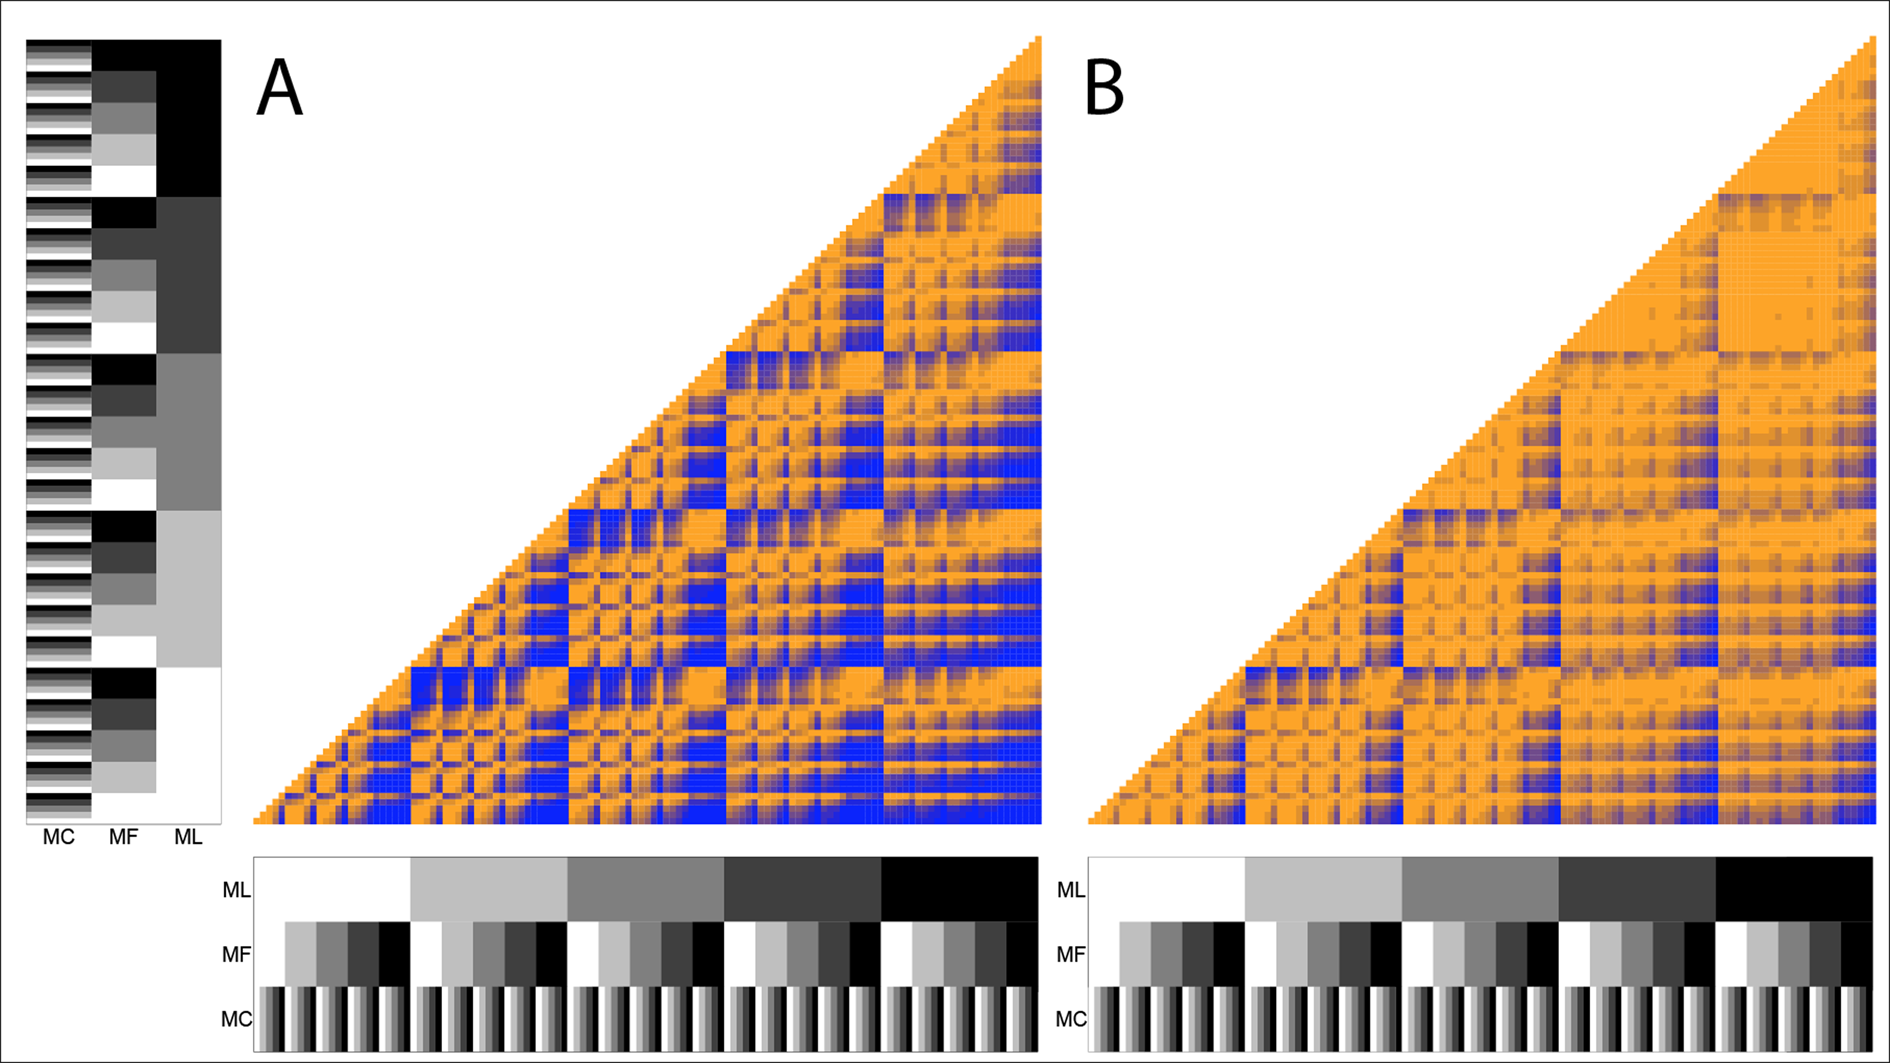
\includegraphics[width=1\textwidth]{OnlineAppendices-LaTeXSuppFiles/SupplementaryFigures/PairwiseComp-Bayt-RF+Tr-colour.png} %bitmap version - 300 dpi RGB
    \caption{The effects of missing data on topological recovery using Bayesian posterior tree distribution. The x and the y axes both show show the percentage of missing data from 0\% (white) to 75\% (black) for the three parameters: $M_{L}$ (upper line), $M_{F}$ (middle line) and $M_{C}$ (lower line). Topological recovery is represented by the probability of (A) Normalised Robinson-Foulds distance and (B) Normalised Triplets distance distributions overlapping with the "best" tree distribution, calculated using the Bhattacharyya Coefficient. TThe Bhattacharyya Coefficient values are indicated using a color gradient ranging from low probability of overlap in blue, to a high probability of overlap in orange.}
\label{Fig_Supp_paircomp_Bayt}
\end{figure} 


%Summary of metrics values for all parameters combinations
\begin{landscape}
\begin{table}[ht]
\caption{Summary of the of the comparisons between the "best" tree and the "missing data" trees for each different tree inference method using either the Normalised Robinson-Foulds distance (RF) or the Normalised Triplets distance (Tr).}
\label{Tab_Supp_summary_metric_allparam}
\centering
\begin{tabular}{lccccccc}
  \hline
 Tree inference method & Metric & Min. & 1st Qu. & Median & Mean & 3rd Qu. & Max. \\ 
  \hline
  Maximum Likelihood                    & $RF$ & 0.06 & 0.26 & 0.40 & 0.41 & 0.50 & 0.95 \\ 
                                        & $Tr$ & 0.29 & 0.45 & 0.59 & 0.63 & 0.84 & 1.00 \\ 
  Bayesian consensus                    & $RF$ & 0.69 & 0.71 & 0.72 & 0.76 & 0.79 & 0.96 \\ 
                                        & $Tr$ & -0.28 & -0.11 & 0.17 & 0.19 & 0.37 & 0.98 \\ 
  Maximum Likelihood bootstraps         & $RF$ & 0.06 & 0.18 & 0.27 & 0.26 & 0.34 & 0.46 \\ 
                                        & $Tr$ & 0.23 & 0.31 & 0.35 & 0.38 & 0.45 & 0.58 \\ 
  Bayesian posterior tree distributions & $RF$ & 0.16 & 0.22 & 0.32 & 0.34 & 0.42 & 0.65 \\ 
                                        & $Tr$ & 0.24 & 0.35 & 0.40 & 0.50 & 0.67 & 0.98 \\ 
   \hline
\end{tabular}
\end{table}
\end{landscape}


%Summary of metrics values for the ML parameter
\begin{landscape}
\begin{table}[ht]
\caption{Summary of the of the comparisons between the "best" tree and the "missing data" trees for each different tree inference method using either the Normalised Robinson-Foulds distance (RF) or the Normalised Triplets distance (Tr) for the $M_{L}$ missing data parameter only.}
\label{Tab_Supp_summary_metric_ML}
\centering
\begin{tabular}{lccccccc}
  \hline
 Tree inference method & Metric & Min. & 1st Qu. & Median & Mean & 3rd Qu. & Max. \\ 
  \hline
  Maximum Likelihood                    & $RF$ & 0.44 & 0.51 & 0.63 & 0.66 & 0.78 & 0.95 \\ 
                                        & $Tr$ & 0.45 & 0.56 & 0.76 & 0.74 & 0.93 & 0.99 \\ 
  Bayesian consensus                    & $RF$ & 0.71 & 0.73 & 0.80 & 0.82 & 0.88 & 0.95 \\ 
                                        & $Tr$ & 0.37 & 0.46 & 0.67 & 0.67 & 0.87 & 0.96 \\ 
  Maximum Likelihood bootstraps         & $RF$ & 0.34 & 0.37 & 0.42 & 0.41 & 0.44 & 0.46 \\ 
                                        & $Tr$ & 0.32 & 0.40 & 0.51 & 0.46 & 0.51 & 0.57 \\ 
  Bayesian posterior tree distributions & $RF$ & 0.33 & 0.41 & 0.52 & 0.50 & 0.60 & 0.65 \\ 
                                        & $Tr$ & 0.41 & 0.56 & 0.76 & 0.71 & 0.84 & 0.98 \\ 
   \hline
\end{tabular}
\end{table}
\end{landscape}


%Summary of metrics values for the MF parameter
\begin{landscape}
\begin{table}[ht]
\caption{Summary of the of the comparisons between the "best" tree and the "missing data" trees for each different tree inference method using either the Normalised Robinson-Foulds distance (RF) or the Normalised Triplets distance (Tr) for the $M_{F}$ missing data parameter only.}
\label{Tab_Supp_summary_metric_MF}
\centering
\begin{tabular}{lccccccc}
  \hline
 Tree inference method & Metric & Min. & 1st Qu. & Median & Mean & 3rd Qu. & Max. \\ 
  \hline
  Maximum Likelihood                    & $RF$ & 0.23 & 0.46 & 0.64 & 0.61 & 0.79 & 0.93 \\ 
                                        & $Tr$ & 0.65 & 0.84 & 0.95 & 0.89 & 0.99 & 1.00 \\ 
  Bayesian consensus                    & $RF$ & 0.72 & 0.77 & 0.86 & 0.85 & 0.94 & 0.96 \\ 
                                        & $Tr$ & -0.16 & 0.19 & 0.63 & 0.52 & 0.96 & 0.98 \\ 
  Maximum Likelihood bootstraps         & $RF$ & 0.14 & 0.30 & 0.40 & 0.35 & 0.45 & 0.46 \\ 
                                        & $Tr$ & 0.37 & 0.49 & 0.54 & 0.51 & 0.56 & 0.57 \\ 
  Bayesian posterior tree distributions & $RF$ & 0.24 & 0.45 & 0.57 & 0.51 & 0.63 & 0.65 \\ 
                                        & $Tr$ & 0.44 & 0.81 & 0.86 & 0.82 & 0.98 & 0.98 \\ 
   \hline
\end{tabular}
\end{table}
\end{landscape}

%Summary of metrics values for the MC parameter
\begin{landscape}
\begin{table}[ht]
\caption{Summary of the of the comparisons between the "best" tree and the "missing data" trees for each different tree inference method using either the Normalised Robinson-Foulds distance (RF) or the Normalised Triplets distance (Tr) for the $M_{C}$ missing data parameter only.}
\label{Tab_Supp_summary_metric_MC}
\centering
\begin{tabular}{lccccccc}
  \hline
 Tree inference method & Metric & Min. & 1st Qu. & Median & Mean & 3rd Qu. & Max. \\ 
  \hline
  Maximum Likelihood                    & $RF$ & 0.40 & 0.50 & 0.64 & 0.65 & 0.79 & 0.94 \\ 
                                        & $Tr$ & 0.70 & 0.84 & 0.93 & 0.89 & 0.99 & 1.00 \\ 
  Bayesian consensus                    & $RF$ & 0.76 & 0.79 & 0.86 & 0.86 & 0.92 & 0.96 \\ 
                                        & $Tr$ & 0.05 & 0.16 & 0.53 & 0.50 & 0.87 & 0.92 \\ 
  Maximum Likelihood bootstraps         & $RF$ & 0.25 & 0.34 & 0.42 & 0.38 & 0.45 & 0.46 \\ 
                                        & $Tr$ & 0.38 & 0.47 & 0.55 & 0.51 & 0.57 & 0.58 \\ 
  Bayesian posterior tree distributions & $RF$ & 0.32 & 0.44 & 0.58 & 0.52 & 0.62 & 0.65 \\ 
                                        & $Tr$ & 0.39 & 0.78 & 0.82 & 0.79 & 0.98 & 0.98 \\ 
   \hline
\end{tabular}
\end{table}
\end{landscape}


%Summary of the BC between pairs of methods for the ML parameter
\begin{landscape}
\begin{table}[ht]
\caption{Bhattacharyya Coefficients of the pairwise method comparisons, each of which corresponds to the normalised distance between the "best" tree and the "missing data" using either the Normalised Robinson-Foulds distance (RF) or the Normalised Triplets distance (Tr) for the $M_{L}$ missing data parameter only.}
\label{Tab_Supp_summary_BC_ML}
\centering
\begin{tabular}{lccccccc}
  \hline
 Comparison &  Metric & Min. & 1st Qu. & Median & Mean & 3rd Qu. & Max. \\ 
  \hline
    Maximum Likelihood \textit{vs.} Bayesian consensus                 & $RF$ & 0.30 & 0.31 & 0.69 & 0.61 & 0.77 & 1.00 \\ 
                                                                       & $Tr$ & 0.79 & 0.81 & 0.84 & 0.86 & 0.85 & 1.00 \\ 
    Maximum Likelihood \textit{vs.} Maximum Likelihood bootstraps      & $RF$ & 0.03 & 0.22 & 0.29 & 0.36 & 0.54 & 0.69 \\ 
                                                                       & $Tr$ & 0.08 & 0.42 & 0.53 & 0.51 & 0.74 & 0.78 \\ 
    Maximum Likelihood \textit{vs.} Bayesian posterior trees           & $RF$ & 0.02 & 0.49 & 0.61 & 0.51 & 0.67 & 0.74 \\ 
                                                                       & $Tr$ & 0.21 & 0.61 & 0.70 & 0.63 & 0.81 & 0.81 \\ 
    Bayesian consensus \textit{vs.} Maximum Likelihood bootstraps      & $RF$ & 0.01 & 0.02 & 0.02 & 0.02 & 0.03 & 0.04 \\ 
                                                                       & $Tr$ & 0.08 & 0.69 & 0.78 & 0.64 & 0.79 & 0.84 \\ 
    Bayesian consensus \textit{vs.} Bayesian posterior trees           & $RF$ & 0.01 & 0.02 & 0.02 & 0.04 & 0.08 & 0.09 \\ 
                                                                       & $Tr$ & 0.21 & 0.74 & 0.75 & 0.68 & 0.84 & 0.87 \\ 
    Bayesian posterior tree \textit{vs.} Maximum Likelihood bootstraps & $RF$ & 0.69 & 0.75 & 0.85 & 0.85 & 0.95 & 1.00 \\ 
                                                                       & $Tr$ & 0.91 & 0.92 & 0.96 & 0.95 & 0.97 & 0.98 \\ 
   \hline
\end{tabular}
\end{table}
\end{landscape}

%Summary of the BC between pairs of methods for the MF parameter
\begin{landscape}
\begin{table}[ht]
\caption{Bhattacharyya Coefficients of the pairwise method comparisons, each of which corresponds to the normalised distance between the "best" tree and the "missing data" using either the Normalised Robinson-Foulds distance (RF) or the Normalised Triplets distance (Tr) for the $M_{F}$ missing data parameter only.}
\label{Tab_Supp_summary_BC_MF}
\centering
\begin{tabular}{lccccccc}
  \hline
 Comparison &  Metric & Min. & 1st Qu. & Median & Mean & 3rd Qu. & Max. \\  
  \hline
    Maximum Likelihood \textit{vs.} Bayesian consensus                 & $RF$ & 0.00 & 0.25 & 0.48 & 0.50 & 0.76 & 1.00 \\ 
                                                                       & $Tr$ & 0.38 & 0.69 & 0.75 & 0.72 & 0.80 & 1.00 \\ 
    Maximum Likelihood \textit{vs.} Maximum Likelihood bootstraps      & $RF$ & 0.03 & 0.18 & 0.32 & 0.36 & 0.47 & 0.77 \\ 
                                                                       & $Tr$ & 0.08 & 0.34 & 0.40 & 0.38 & 0.53 & 0.55 \\ 
    Maximum Likelihood \textit{vs.} Bayesian posterior trees           & $RF$ & 0.02 & 0.47 & 0.71 & 0.60 & 0.86 & 0.94 \\ 
                                                                       & $Tr$ & 0.21 & 0.54 & 0.62 & 0.56 & 0.64 & 0.80 \\ 
    Bayesian consensus \textit{vs.} Maximum Likelihood bootstraps      & $RF$ & 0.00 & 0.00 & 0.01 & 0.01 & 0.01 & 0.03 \\ 
                                                                       & $Tr$ & 0.08 & 0.38 & 0.54 & 0.49 & 0.70 & 0.75 \\ 
    Bayesian consensus \textit{vs.} Bayesian posterior trees           & $RF$ & 0.00 & 0.02 & 0.02 & 0.02 & 0.04 & 0.04 \\ 
                                                                       & $Tr$ & 0.21 & 0.29 & 0.66 & 0.54 & 0.72 & 0.82 \\ 
    Bayesian posterior tree \textit{vs.} Maximum Likelihood bootstraps & $RF$ & 0.69 & 0.69 & 0.72 & 0.71 & 0.72 & 0.72 \\ 
                                                                       & $Tr$ & 0.91 & 0.91 & 0.91 & 0.93 & 0.92 & 0.98 \\ 
   \hline
\end{tabular}
\end{table}
\end{landscape}

%Summary of the BC between pairs of methods for the MC parameter
\begin{landscape}
\begin{table}[ht]
\caption{Bhattacharyya Coefficients of the pairwise method comparisons, each of which corresponds to the normalised distance between the "best" tree and the "missing data" using either the Normalised Robinson-Foulds distance (RF) or the Normalised Triplets distance (Tr) for the $M_{C}$ missing data parameter only.}
\label{Tab_Supp_summary_BC_MC}
\centering
\begin{tabular}{lccccccc}
  \hline
 Comparison &  Metric & Min. & 1st Qu. & Median & Mean & 3rd Qu. & Max. \\  
  \hline
    Maximum Likelihood \textit{vs.} Bayesian consensus                 & $RF$ & 0.03 & 0.32 & 0.66 & 0.55 & 0.75 & 1.00 \\ 
                                                                       & $Tr$ & 0.51 & 0.69 & 0.80 & 0.76 & 0.80 & 1.00 \\ 
    Maximum Likelihood \textit{vs.} Maximum Likelihood bootstraps      & $RF$ & 0.03 & 0.17 & 0.21 & 0.31 & 0.46 & 0.68 \\ 
                                                                       & $Tr$ & 0.08 & 0.31 & 0.39 & 0.39 & 0.56 & 0.61 \\ 
    Maximum Likelihood \textit{vs.} Bayesian posterior trees           & $RF$ & 0.02 & 0.44 & 0.47 & 0.52 & 0.78 & 0.90 \\ 
                                                                       & $Tr$ & 0.21 & 0.52 & 0.59 & 0.55 & 0.66 & 0.77 \\ 
    Bayesian consensus \textit{vs.} Maximum Likelihood bootstraps      & $RF$ & 0.00 & 0.01 & 0.01 & 0.02 & 0.02 & 0.03 \\ 
                                                                       & $Tr$ & 0.08 & 0.47 & 0.62 & 0.51 & 0.66 & 0.73 \\ 
    Bayesian consensus \textit{vs.} Bayesian posterior trees           & $RF$ & 0.00 & 0.02 & 0.04 & 0.04 & 0.05 & 0.06 \\ 
                                                                       & $Tr$ & 0.21 & 0.45 & 0.64 & 0.57 & 0.74 & 0.79 \\ 
    Bayesian posterior tree \textit{vs.} Maximum Likelihood bootstraps & $RF$ & 0.69 & 0.73 & 0.73 & 0.76 & 0.81 & 0.86 \\ 
                                                                       & $Tr$ & 0.91 & 0.92 & 0.93 & 0.94 & 0.96 & 0.99 \\ 
   \hline
\end{tabular}
\end{table}
\end{landscape}
  \label{Supp_results}

%END
\end{document}